\documentclass[a4paper,11pt]{article}
\usepackage[T1]{fontenc}
\usepackage[utf8]{inputenc}
\usepackage{lmodern}
\usepackage[francais]{babel}

\usepackage{listings}

%couleur
\usepackage{color}
\usepackage{multicol}

%image
\usepackage{graphicx}

\definecolor{ligthyellow}{RGB}{250,247,220}
\definecolor{darkblue}{RGB}{5,10,85}
\definecolor{ligthblue}{RGB}{1,147,128}
\definecolor{darkgreen}{RGB}{8,120,51}
\definecolor{darkred}{RGB}{160,0,0}
\definecolor{univ}{RGB}{177,23,119}
\definecolor{univmodif}{RGB}{148,74,120}
\definecolor{mygray}{RGB}{100,100,100}

\lstset{
    language=Python,
    captionpos=b,
    extendedchars=true,
    frame=lines,
    numbers=left,
    numberstyle=\tiny,
    numbersep=5pt,
    keepspaces=true,
    breaklines=true,
    showspaces=false,
    showstringspaces=false,
    breakatwhitespace=false,
    stepnumber=1,
    showtabs=false,
    tabsize=3,
    basicstyle=\small\ttfamily,
    backgroundcolor=\color{ligthyellow},
    keywordstyle=\color{ligthblue},
    morekeywords={include, printf, uchar},
    identifierstyle=\color{darkblue},
    commentstyle=\color{darkgreen},
    stringstyle=\color{darkred},
}

\title{Logique flou pour la segmentation d'image couleur}
\author{Elliot Vanegue}

\begin{document}

\maketitle
%\tableofcontents

%\begin{abstract}
%\end{abstract}

\section{Introduction}
Nous avons vu dans le TP précédent ce qu'était la logique floue au travers d'exemple ne portant pas 
sur la segmentation d'image. La logique floue permet en effet d'avoir un niveau d'incertitude sur 
l'appartenance d'une donnée à une classe. Dans ce TP, nous allons voir comment appliquer cette méthode
à la segmentation d'image couleur. Par la suite, nous verrons différentes méthodes dérivées du 
principe de la logique floue afin de comparer leur performance. Tout au long de ce TP, nous utilisons
l'image de la Fig. \ref{fig:reference}.

\begin{figure}[!h]
  \begin{center}
    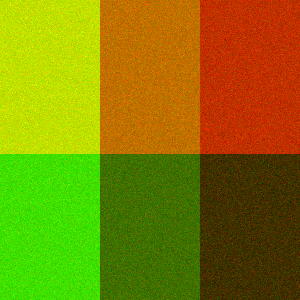
\includegraphics[width=5cm]{6_classes_RGB.png}
    \caption{Image de référence du TP}
    \label{fig:reference}
  \end{center}
\end{figure}

\section{FCM (Fuzzy C-Means)}
Dans un premier temps nous utiliser la méthode de la logique floue pour segmenter une image couleur. 
Cette méthode est très proche de l'algorithme du K-means. La différence entre les deux algorithme
est que dans l'algorithme FCM une donnée n'appartient pas à une classe, mais elle a une certaine
probabilité d'y appartenir. Tout comme pour K-means, l'algorithme a besoin d'un certain nombre de
paramètre pour fonctionner. Ces paramètres sont fournis par l'utilisateur.
\begin{itemize}
  \item c : le nombre de classe à segmenter. Ce paramètre détermine le nombre de centroïde à créer.
  \item m : le degré d'appartenance d'une donnée. Ce paramètre permet d'avoir un plus ou moins grand écart
  entre les taux d'appartenances aux classes. Plus il sera élevé plus l'appartenance d'une donnée à une classe
  est forte. Cependant, si m est trop élevé, la correction des erreurs par les étapes suivantes est plus difficile.
  \item seuil : le seuil de stabilité à partir de laquelle l'algorithme peut s’arrêter.
\end{itemize}
Au début de l'algorithme, les centroïdes sont placés aléatoirement parmi les données. Puis à chaque itération,
ces centoïdes se rapproche du centre d'un ensemble de données tout en s'éloignant les uns des autres. La détermination
de la position des centroïdes se fait grâce au calcul (Eq. \ref{centroide}).
\begin{equation}
  \label{centroide}
  \forall i \in \{1, 2, ..., c\} \ v_i = \frac{\sum_{j=1}^{n} u_{ij}^m * x_j}{\sum_{j=1}^{n} u_{ij}^m}
\end{equation}
Dans cette équation, n est le nombre de pixels. La matrice $u$ représente
le degré d'appartenance des pixels pour une classe. Il est possible de calculer cette matrice avec l'équation
(Eq. \ref{membershipDegree}).
\begin{equation}
 \label{membershipDegree}
  u_{ij}=\left[\sum_{k=1}^{c} \left(\frac{d^2(x_j, v_i)}{d^2(x_j, v_k)}\right)^{\frac{2}{m-1}}\right]^{-1}
\end{equation}
Ces deux calculs permettent donc de placer les centroïde au centre des classes détecté. Il faut maintenant permettre
à l'algorithme de s’arrêter lorsque le seuil de stabilité est atteint. Pour cela, il faut calculer la performance
de l'étape qui a été calculé, c'est-à-dire qu'il faut minimiser le taux d'appartenance des pixels par la distance
avec le centroïde (Eq. \ref{jp}) et comparer ce résultat avec celui de l'étape précédente (Eq. \ref{jpMin}).

\begin{equation}
  \label{jp}
  J_{FCM}(P)=\sum_{i=1}^{c}\sum_{j=1}^{n}[u_{ij}]^m * d_{ij}^2
\end{equation}

\begin{equation}
  \label{jpMin} 
  J_{FCM}(P) - J_{FCM}(P-1) < seuil
\end{equation}

Nous obtenons la segmentation de la Fig. \ref{fig:segmentationFCM}, qui nous permet d'avoir
un résultat très intéressant. On peut voir sur la courbe représentant $J_{FCM}(P)$ (Fig. \ref{fig:graphFCM}), que l'algorithme
fonctionne en très peu d'étape et que dès la première étape il est très proche du bon résultat.

\begin{figure}[!h]
  \begin{center}
    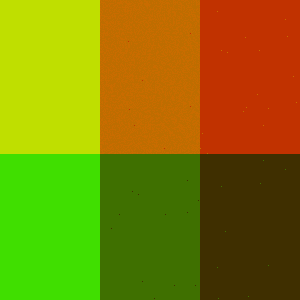
\includegraphics[width=5cm]{resultat/FCM.png}
    \caption{Résultat de la segmentation d'une image couleur avec l'algorithme FCM}
    \label{fig:segmentationFCM}
  \end{center}
\end{figure}

\begin{figure}[!h]
  \begin{center}
    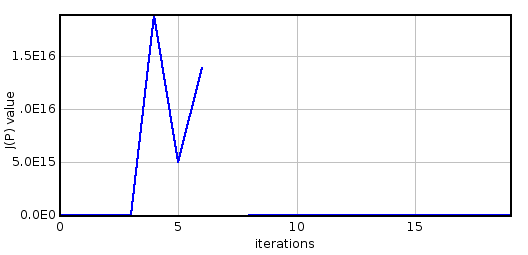
\includegraphics[width=7cm]{resultat/FCM_graph.png}
    \caption{Graphique de $J_{FCM}(P)$}
    \label{fig:graphFCM}
  \end{center}
\end{figure}

\section{HCM (Hard C-Means)}
L'algorithme HCM est similaire à l'algorithme K-means. Il n'utilise pas de degré d'appartenance
d'une donnée à une classe, soit la donnée appartient à une classe, soit elle n'y appartient pas.
Le changement majeur dans l'algorithme du FCM est donc le calcul de $u_{ij}$. Pour déterminer à quel
classe appartient une donnée on compare avec la distance de sa coordonnée avec chaque centroïde et
on choisit la classe ayant la plus courte distance. Cela nous fournit le résultat de la Fig. \ref{fig:hcm}.\\

\begin{figure}[!h]
  \begin{center}
    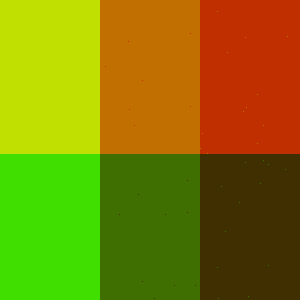
\includegraphics[width=5cm]{resultat/HCM.png}
    \caption{Résultat de la segmentation d'une image couleur avec l'algorithme HCM}
    \label{fig:hcm}
  \end{center}
\end{figure}

\begin{figure}[!h]
  \begin{center}
    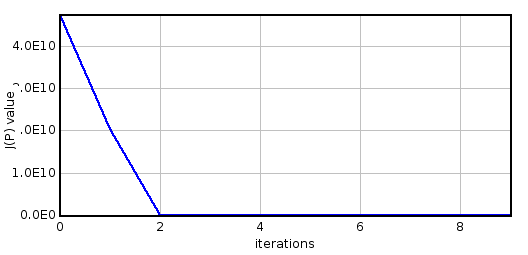
\includegraphics[width=7cm]{resultat/HCM_graph.png}
    \caption{Graphique de $J_{HCM}(P)$}
    \label{fig:graphHCM}
  \end{center}
\end{figure}

Encore une fois, la segmentation est efficace, même si la première étape est moins performante, l'algorithme
se termine en deux étapes.
\newpage
\section{PCM (Possibilistic C-Means)}
L'algorithme PCM fonctionne sur le même principe que le FCM tout en introduisant une valeur de pénalité
sur l'appartenance d'une donnée à une classe. Le calcul de cette pénalité est calculé dans l'Eq. \ref{penalite}.

\begin{equation}
  \label{penalite}
  \eta_i = \frac{\sum_{j=1}^{n} u_{ij}^m * x_j}{\sum_{j=1}^{n} u_{ij}^m}
\end{equation}

Cette pénalité est appliqué au calcul de $u_ij$ et à la performance de l'étape courante.

\begin{equation}
  \label{uijPCM}
  \eta_i = \frac{\sum_{j=1}^{n} u_{ij}^m * x_j}{\sum_{j=1}^{n} u_{ij}^m}
\end{equation}

\newpage
\section{Annexes}
\begin{lstlisting}[caption=Algorithme FCM]
   imax = nbpixels;  // nombre de pixels dans l image
   jmax = 3;  // nombre de composantes couleur
	kmax=nbclasses;
	double data[][] = new double[nbclasses][3];
	int[] fixe=new int[3];
	int xmin = 0;
	int xmax = width;
	int ymin = 0;
	int ymax = height;
	int rx, ry;
	int x,y;
	int epsilonx,epsilony;


	// Initialisation des centroides (aleatoirement )
	for(i=0;i<nbclasses;i++)
	{
		if(valeur==1)
		{
			epsilonx=rand((int)(width/(i+2)),(int)(width/2));
			epsilony=rand((int)(height/(4)),(int)(height/2));
		}
		else
		{
			epsilonx=0;
			epsilony=0;
		}
		rx = rand(xmin+epsilonx, xmax-epsilonx);
		ry = rand(ymin+epsilony, ymax-epsilony);
		ip.getPixel(rx,ry,init);
		c[i][0] = init[0]; c[i][1] =init[1]; c[i][2] = init[2];
	}

	// Calcul de distance entre data et centroides
	for(l = 0; l < nbpixels; l++)
	{
		for(k = 0; k < kmax; k++)
		{
			double r2 = Math.pow(red[l] - c[k][0], 2);
			double g2 = Math.pow(green[l] - c[k][1], 2);
			double b2 = Math.pow(blue[l] - c[k][2], 2);
			Dprev[k][l] = r2 + g2 + b2;
		}
	}

	// Initialisation des degres d'appartenance
	float membership = 0.0f;
  for(i = 0 ; i < kmax ; i++){
      for(j = 0 ; j < nbpixels ; j++){
          membership = 0.0f;
          for(k = 1 ; k < kmax ; k++){
							if(Math.pow(Dprev[k][j], 2) < 1)
								continue;
              membership += Math.pow( Math.pow(Dprev[i][j], 2) / Math.pow(Dprev[k][j], 2), 2/(m-1) );
          }
          Uprev[i][j] = Math.pow(membership, -1);
					if(Uprev[i][j] > 1)
						Uprev[i][j] = 1/Uprev[i][j];
      }
  }

	/////////////////////////////////////////////////////////////
	// BOUCLE PRINCIPALE
	////////////////////////////////////////////////////////////
	iter = 0;
	stab = 2;
	seuil = valeur_seuil;
	
	while ((iter < itermax) && (stab > seuil))
	{
		// Update  the matrix of centroids
		float num[] = new float[3];
		float den;
		for(k = 0 ; k < kmax ; k++){
			num[0] = 0.0f;
			num[1] = 0.0f;
			num[2] = 0.0f;
			den = 0.0f;
      for(i = 0 ; i < nbpixels ; i++){
      	num[0] += Math.pow(Uprev[k][i],m) * (double)red[i];
      	num[1] += Math.pow(Uprev[k][i],m) * (double)green[i];
      	num[2] += Math.pow(Uprev[k][i],m) * (double)blue[i];
      	den += Math.pow(Uprev[k][i],m);
      }

      c[k][0] = num[0] / den;
      c[k][1] = num[1] / den;
      c[k][2] = num[2] / den;
  	}
		// Compute Dmat, the matrix of distances (euclidian) with the centroids
		for(l = 0; l < nbpixels; l++)
		{
			for(k = 0; k < kmax; k++)
			{
				double r2 = Math.pow(red[l] - c[k][0], 2);
				double g2 = Math.pow(green[l] - c[k][1], 2);
				double b2 = Math.pow(blue[l] - c[k][2], 2);
				Dmat[k][l] = r2 + g2 + b2;
			}
		}

		for(i = 0 ; i < kmax ; i++){
			for(j = 0 ; j < nbpixels ; j++){
				for(k = 1 ; k < kmax ; k++){
					if(Math.pow(Dmat[k][j], 2) == 0)
						continue;
					Umat[i][j] += Math.pow( Dmat[i][j] / Dmat[k][j], (2/(m-1)) );
				}
				if(Umat[i][j] > 1)
					Umat[i][j] = 1/Umat[i][j];
			}
		}

		for(i = 0 ; i < kmax ; i++){
			for(j = 0 ; j < nbpixels ; j++){
				Uprev[i][j] = Umat[i][j];
				Dprev[i][j] = Dmat[i][j];
			}
		}

		// Calculate difference between the previous partition and the new partition (performance index)
		for(i = 0 ; i < kmax ; i++){
			for(j = 0 ; j < nbpixels ; j++){
				figJ[iter] += Math.pow(Umat[i][j], m) * Math.pow(Dmat[i][j], 2);
			}
		}

		if(iter > 0)
			stab = figJ[iter] - figJ[iter-1];

		iter++;
		////////////////////////////////////////////////////////

		// Affichage de l'image segmentee
		double[] mat_array=new double[nbclasses];
		l = 0;
		for(i=0;i<width;i++)
		{
			for(j = 0; j<height; j++)
			{
				for(k = 0; k<nbclasses; k++)
				{
					mat_array[k]=Umat[k][l];
				}
				int indice= IndiceMaxOfArray(mat_array,nbclasses) ;
				int array[] = new int[3];
				array[0] = (int)c[indice][0];
				array[1] = (int)c[indice][1];
				array[2] = (int)c[indice][2];
				ipseg.putPixel(i, j, array);
				l++;
			}
		}
		impseg.updateAndDraw();
		
	}  

	double[] xplot= new double[itermax];
	double[] yplot=new double[itermax];
	for(int w = 0; w < itermax; w++)
	{
		xplot[w]=(double)w;	yplot[w]=(double) figJ[w];
	}
	Plot plot = new Plot("Performance Index (FCM)","iterations","J(P) value",xplot,yplot);
	plot.setLineWidth(2);
	plot.setColor(Color.blue);
	plot.show();
}
\end{lstlisting}
  
\end{document}
